\chapter{Environnement Laboratoire}
\label{chap:labo}

\section{Outils utilisés}

\subsection{GNS3}

GNS3 (Graphical Network Simulator-3) est un simulateur réseau open source permettant de reproduire des architectures réseau complexes \cite{6}. Il supporte :
\begin{itemize}
    \item Les émulateurs QEMU/KVM pour les VMs (FortiGate, Ubuntu)
    \item Les conteneurs Docker pour les services légers
    \item Les switches Open vSwitch (OVS) pour le switching L2
    \item La simulation de liens physiques et de VLANs
\end{itemize}

\subsection{QEMU/KVM}

QEMU avec KVM (Kernel-based Virtual Machine) fournit l'émulation matérielle des FortiGate. Le support KVM assure des performances proches du natif, avec un accès direct au processeur hôte.

\subsection{Docker}

Docker permet le déploiement rapide de services légers :
\begin{itemize}
    \item \textbf{PostgreSQL} : base de données relationnelle
    \item \textbf{appServer} : serveur d'application Flask
    \item \textbf{Grafana} : tableaux de bord de supervision
    \item \textbf{Prometheus} : collecte de métriques
    \item \textbf{Traffic-Gen} : génération de trafic et syslog
    \item \textbf{Alpine DHCP} : serveur DHCP pour LAN2
    \item \textbf{OpenvSwitch} : switches virtuels L2
    \item \textbf{Docker Router} : routeur cross-LAN
\end{itemize}

\subsection{Open vSwitch (OVS)}

Open vSwitch est un switch virtuel open source offrant le support VLAN 802.1Q, le trunking, et la gestion des bridges. Deux instances OVS sont déployées pour isoler les segments LAN1 et LAN2.

\section{Topologie réseau}

\subsection{Architecture modifiée}

La topologie modifiée du laboratoire comprend 4 pare-feux FortiGate organisés en 2 paires HA, avec un routeur Docker pour le routage inter-LAN :

\begin{itemize}
    \item \textbf{FGT-Primary (ACTIF)} : pare-feu principal LAN1
    \item \textbf{FGT-Primary-HA (STANDBY)} : backup de FGT-Primary
    \item \textbf{FGT-Secondary (ACTIF)} : pare-feu principal LAN2
    \item \textbf{FGT-Secondary-HA (STANDBY)} : backup de FGT-Secondary
    \item \textbf{Docker Router} : routage cross-LAN entre LAN1 et LAN2
\end{itemize}

\begin{figure}[H]
\centering
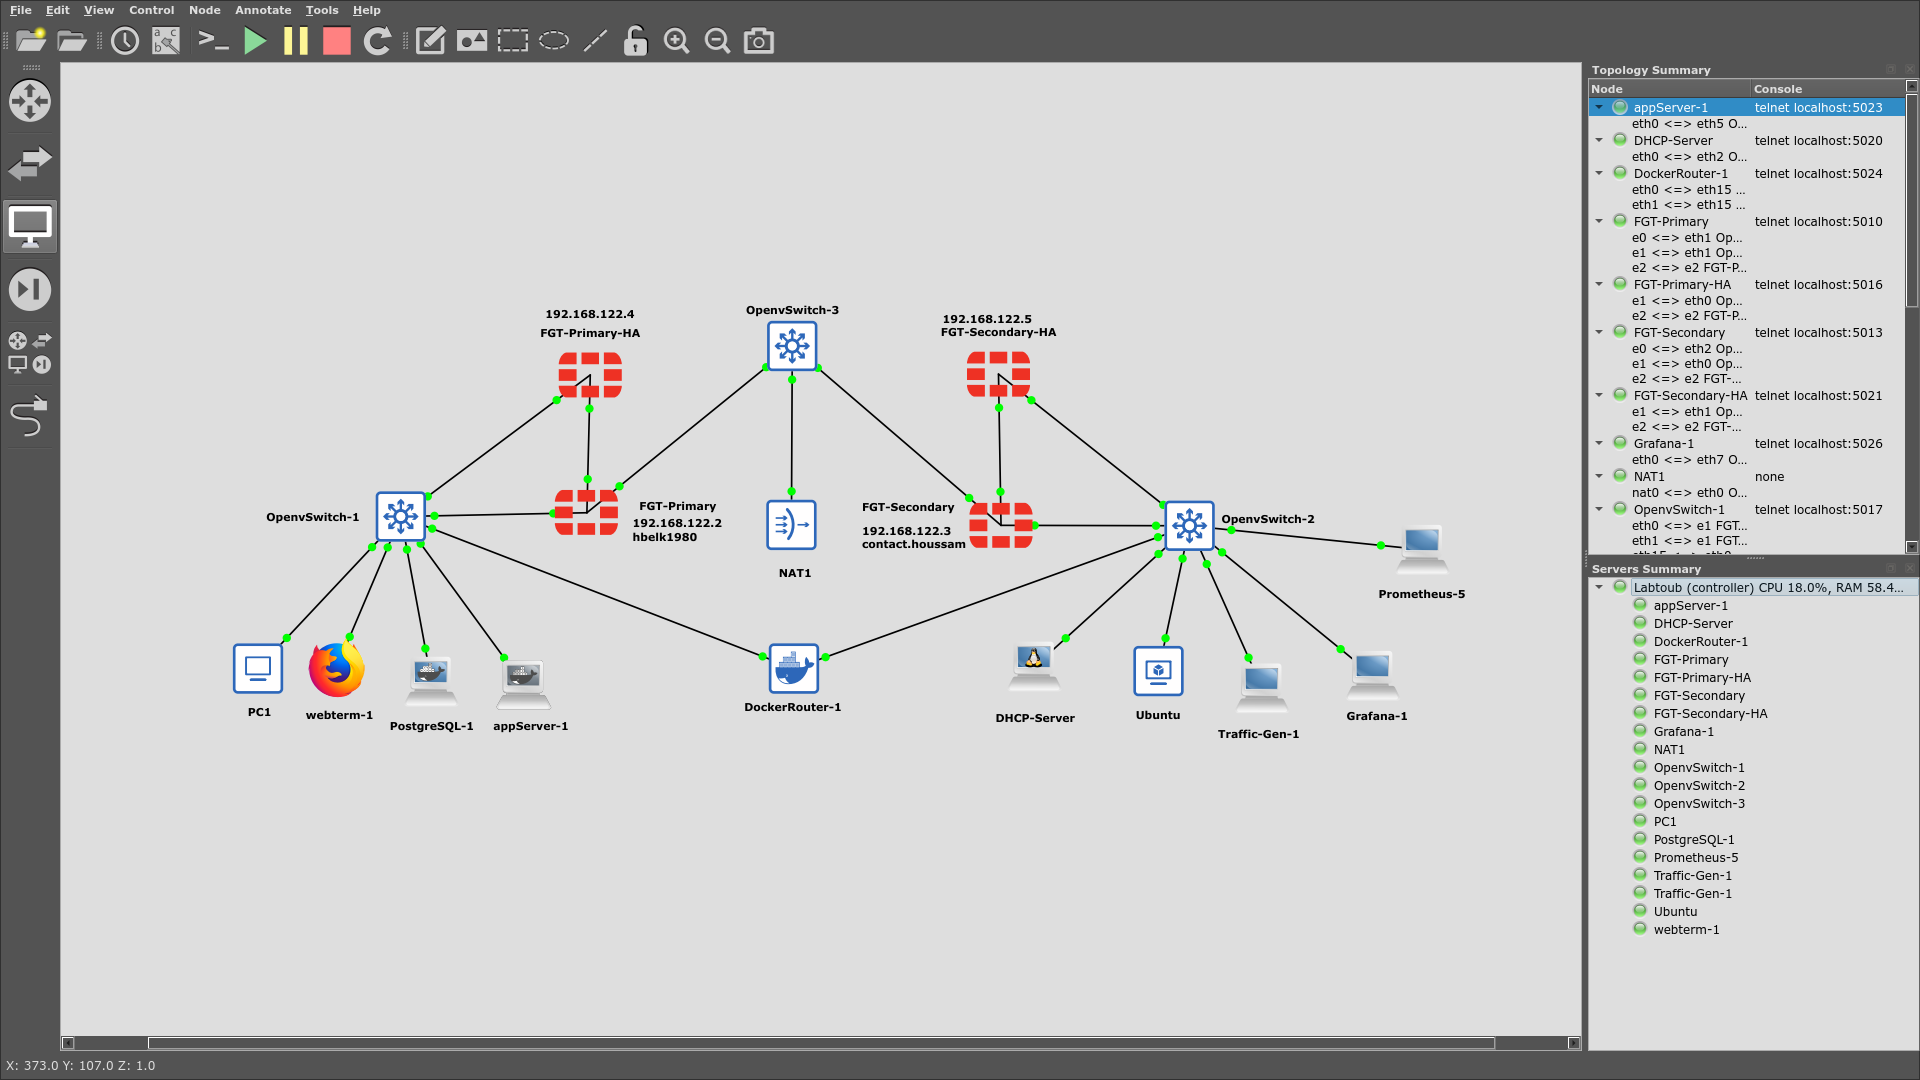
\includegraphics[width=0.9\textwidth]{images/topo-gns3.png}
\caption{Topologie GNS3 modifiée --- Vue d'ensemble}
\label{fig:topo-gns3}
\end{figure}

\subsection{Principes de conception}

\begin{itemize}
    \item \textbf{Pas de transit OSPF} : le lien transit entre les FGT a été remplacé par un Docker Router, libérant le port3 pour le heartbeat HA
    \item \textbf{Isolation LAN} : OVS-LAN1 et OVS-LAN2 sont complètement séparés
    \item \textbf{HA Active-Passive} : chaque pare-feu a un backup sur le même segment
\end{itemize}

\section{Plan d'adressage IP}

\begin{table}[H]
\centering
\caption{Plan d'adressage IP}
\label{tab:adressage-ip}
{\small
\begin{tabularx}{\textwidth}{|l|l|l|X|}
\hline
\textbf{Segment} & \textbf{Subnet} & \textbf{Passerelle} & \textbf{DHCP} \\
\hline
WAN (NAT1) & 192.168.122.0/24 & 192.168.122.1 (virbr0) & virbr0/libvirt \\
\hline
LAN1 (FGT-Primary) & 192.168.10.0/24 & 192.168.10.1 (FGT-P port2) & FGT-Primary (100-200) \\
\hline
LAN2 (FGT-Secondary) & 192.168.20.0/24 & 192.168.20.1 (FGT-S port2) & Alpine DHCP (100-200) \\
\hline
HA Heartbeat & 169.254.0.0/30 & --- (point-a-point) & Statique \\
\hline
\end{tabularx}
}
\end{table}

\subsection{Adressage statique}

\begin{table}[H]
\centering
\caption{Adressage statique des nodes}
\label{tab:static-ip}
\begin{tabularx}{\textwidth}{|l|l|X|}
\hline
\textbf{Node} & \textbf{IP} & \textbf{Segment} \\
\hline
FGT-Primary port1 & DHCP (192.168.122.x) & WAN \\
FGT-Primary port2 & 192.168.10.1/24 & LAN1 \\
FGT-Primary port3 & 169.254.0.1/30 & HA Heartbeat \\
\hline
FGT-Secondary port1 & DHCP (192.168.122.x) & WAN \\
FGT-Secondary port2 & 192.168.20.1/24 & LAN2 \\
FGT-Secondary port3 & 169.254.0.2/30 & HA Heartbeat \\
\hline
Docker Router eth0 & 192.168.10.254/24 & LAN1 \\
Docker Router eth1 & 192.168.20.254/24 & LAN2 \\
\hline
Alpine DHCP & 192.168.20.2/24 & LAN2 \\
App-Server & 192.168.10.10/24 & LAN1 \\
PostgreSQL & 192.168.10.11/24 & LAN1 \\
Grafana & 192.168.20.11/24 & LAN2 \\
Prometheus & 192.168.20.12/24 & LAN2 \\
Traffic-Gen & 192.168.20.10/24 & LAN2 \\
\hline
\end{tabularx}
\end{table}

\section{Spécifications des nodes}

\subsection{VMs QEMU}

\begin{table}[H]
\centering
\caption{Spécifications des VMs QEMU}
\label{tab:qemu-specs}
\begin{tabularx}{\textwidth}{|l|c|c|c|l|X|}
\hline
\textbf{Node} & \textbf{RAM} & \textbf{vCPU} & \textbf{Adaptateurs} & \textbf{Console} & \textbf{Image} \\
\hline
FGT-Primary & 2 GB & 1 & 8 (3 utilisables) & Telnet & fgt-v7.4.12.qcow2 \\
FGT-Primary-HA & 2 GB & 1 & 8 (3 utilisables) & Telnet & fortios.qcow2 (7.0.9) \\
FGT-Secondary & 2 GB & 1 & 8 (3 utilisables) & Telnet & fgt-v7.4.12.qcow2 \\
FGT-Secondary-HA & 2 GB & 1 & 8 (3 utilisables) & Telnet & fortios.qcow2 (7.0.9) \\
Ubuntu Desktop & 2 GB & 2 & 1 (e1000) & VNC & ubuntu-24.04-cloudimg \\
\hline
\end{tabularx}
\end{table}

\subsection{Nodes Docker}

\begin{table}[H]
\centering
\caption{Spécifications des nodes Docker}
\label{tab:docker-specs}
\begin{tabularx}{\textwidth}{|l|l|c|l|X|}
\hline
\textbf{Node} & \textbf{Image} & \textbf{Adaptateurs} & \textbf{Console} & \textbf{Rôle} \\
\hline
OVS-LAN1 & gns3/openvswitch & 16 & Telnet & Switch L2 LAN1 \\
OVS-LAN2 & gns3/openvswitch & 16 & Telnet & Switch L2 LAN2 \\
Docker Router & frrouting/frr & 2 & Telnet & Routage cross-LAN \\
Alpine-DHCP & alpine-dhcp & 1 & Telnet & DHCP LAN2 \\
appServer-1 & python:3.12-alpine & 1 & Telnet & Serveur Flask \\
PostgreSQL-1 & postgres:16-alpine & 1 & Telnet & Base de données \\
Grafana-1 & grafana/grafana & 1 & VNC & Dashboards \\
Prometheus-1 & prom/prometheus & 1 & VNC & Métriques \\
Traffic-Gen-1 & alpine:latest & 1 & Telnet & Syslog + menaces \\
\hline
\end{tabularx}
\end{table}

\subsection{Nodes intégrés GNS3}

\begin{table}[H]
\centering
\caption{Nodes intégrés GNS3}
\label{tab:builtin-specs}
\begin{tabularx}{\textwidth}{|l|l|X|}
\hline
\textbf{Node} & \textbf{Type} & \textbf{Rôle} \\
\hline
PC1 & VPCS & Client CLI sur LAN1 \\
NAT1 & Cloud (virbr0) & Passerelle WAN 192.168.122.1 \\
Switch1 & Ethernet switch & Distribution WAN \\
\hline
\end{tabularx}
\end{table}

\section{Câblage et connectique}

\subsection{Câblage FGT-Primary}

\begin{table}[H]
\centering
\caption{Câblage FGT-Primary}
\label{tab:cable-fgtp}
\begin{tabularx}{\textwidth}{|l|l|l|X|}
\hline
\textbf{Port FGT} & \textbf{Adaptateur} & \textbf{Connecté à} & \textbf{IP} \\
\hline
port1 & a0p0 & Switch1 a0p1 & DHCP \\
port2 & a1p0 & OVS-LAN1 a0p0 & 192.168.10.1/24 \\
port3 & a2p0 & FGT-Primary-HA a2p0 & 169.254.0.1/30 \\
\hline
\end{tabularx}
\end{table}

\subsection{Câblage FGT-Secondary}

\begin{table}[H]
\centering
\caption{Câblage FGT-Secondary}
\label{tab:cable-fgts}
\begin{tabularx}{\textwidth}{|l|l|l|X|}
\hline
\textbf{Port FGT} & \textbf{Adaptateur} & \textbf{Connecté à} & \textbf{IP} \\
\hline
port1 & a0p0 & Switch1 a0p2 & DHCP \\
port2 & a1p0 & OVS-LAN2 a0p0 & 192.168.20.1/24 \\
port3 & a2p0 & FGT-Secondary-HA a2p0 & 169.254.0.2/30 \\
\hline
\end{tabularx}
\end{table}

\subsection{Câblage OVS-LAN1}

\begin{table}[H]
\centering
\caption{Câblage OVS-LAN1}
\label{tab:cable-ovs1}
\begin{tabularx}{\textwidth}{|l|l|X|}
\hline
\textbf{Port OVS} & \textbf{Connecté à} & \textbf{Rôle} \\
\hline
eth0 & FGT-Primary a1p0 & Upstream firewall \\
eth1 & PC1 a0p0 & Client VPCS \\
eth2 & appServer-1 a0p0 & Serveur Flask \\
eth3 & PostgreSQL-1 a0p0 & Base de données \\
eth4 & Docker Router eth0 & Routeur cross-LAN \\
\hline
\end{tabularx}
\end{table}

\subsection{Câblage OVS-LAN2}

\begin{table}[H]
\centering
\caption{Câblage OVS-LAN2}
\label{tab:cable-ovs2}
\begin{tabularx}{\textwidth}{|l|l|X|}
\hline
\textbf{Port OVS} & \textbf{Connecté à} & \textbf{Rôle} \\
\hline
eth0 & FGT-Secondary a1p0 & Upstream firewall \\
eth1 & Alpine-DHCP a0p0 & Serveur DHCP \\
eth2 & Ubuntu Desktop a0p0 & Client bureau \\
eth3 & Traffic-Gen a0p0 & Génération trafic \\
eth4 & Grafana a0p0 & Dashboards \\
eth5 & Prometheus a0p0 & Métriques \\
eth6 & Docker Router eth1 & Routeur cross-LAN \\
\hline
\end{tabularx}
\end{table}

\section{Contraintes de la licence eval}

Les FortiGate en licence d'évaluation présentent des limites strictes qui ont influencé la conception du laboratoire :

\begin{table}[H]
\centering
\caption{Limites de la licence eval FortiGate}
\label{tab:eval-limits}
\begin{tabularx}{\textwidth}{|l|l|X|}
\hline
\textbf{Ressource} & \textbf{Limite} & \textbf{Impact sur le labo} \\
\hline
Interfaces & 3 (port1, port2, port3) & WAN + LAN + HA Heartbeat \\
\hline
Firewall policies & 3 & Design compact des règles \\
\hline
Routes & 3 & Routage minimal \\
\hline
vCPU & 1 & performances limitées \\
\hline
RAM & 2 GB & charge réduite \\
\hline
VDOMs & 2 (root + 1 traffic) & non utilisés \\
\hline
Chiffrement & Bas uniquement & AES128-SHA256, DH14 \\
\hline
\end{tabularx}
\end{table}

\noindent\textit{Conséquence majeure :} Avec 3 ports uniquement, le port3 doit être partagé entre le heartbeat HA et le routage inter-LAN. La topologie modifiée résout ce problème en utilisant un Docker Router pour le routage cross-LAN, libérant le port3 exclusivement pour le heartbeat HA.

\section{Architecture hôte}

Le laboratoire s'exécute sur une station de travail sous \textbf{Arch Linux} avec les caractéristiques suivantes :

\begin{itemize}
    \item \textbf{OS} : Arch Linux (noyau Linux)
    \item \textbf{Virtualisation} : QEMU/KVM via GNS3
    \item \textbf{Docker} : serveur Docker avec bridge network \texttt{fortigate-lab}
    \item \textbf{GNS3} : serveur local (gns3server)
\end{itemize}

\section{Budget ressources}

\begin{table}[H]
\centering
\caption{Budget ressources hôte}
\label{tab:resource-budget}
\begin{tabularx}{\textwidth}{|l|l|c|X|}
\hline
\textbf{Composant} & \textbf{RAM} & \textbf{Nombre} & \textbf{Total} \\
\hline
FGT-Primary & 2048 MB & 1 & 2048 MB \\
FGT-Primary-HA & 2048 MB & 1 & 2048 MB \\
FGT-Secondary & 2048 MB & 1 & 2048 MB \\
FGT-Secondary-HA & 2048 MB & 1 & 2048 MB \\
Ubuntu Desktop & 2048 MB & 1 & 2048 MB \\
Conteneurs Docker & $\approx$ 64 MB & 8 & $\approx$ 512 MB \\
Serveur GNS3 + overhead & --- & --- & $\approx$ 512 MB \\
\hline
\textbf{Total} & & & \textbf{$\approx$ 9,3 GB} \\
\hline
\end{tabularx}
\end{table}
